\documentclass[12pt]{article}
\usepackage{amsmath, amsthm, amssymb}
\usepackage{tikz}
\usepackage{geometry}
\usepackage{enumitem}

\geometry{margin=1in}

% Theorem environments
\theoremstyle{definition}
\newtheorem{definition}{Definition}

\theoremstyle{plain}
\newtheorem{theorem}{Theorem}

% Shorthand
\newcommand{\BT}{binary tree}
\newcommand{\FBT}{full binary tree}

\title{\textbf{Leaves vs.\ Internal Nodes in a Full Binary Tree}}
\author{}
\date{}

\begin{document}
\maketitle

% ─────────────────────────────────────────────
\begin{definition}
A \textbf{binary tree} is called \textbf{full} if every node has either $0$ or $2$ children.
\end{definition}

% ─────────────────────────────────────────────
\paragraph{Example.}
The following is a full binary tree with $3$ internal nodes and $4$ leaves:

\begin{center}
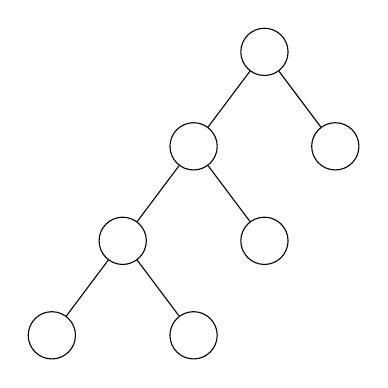
\begin{tikzpicture}[
  every node/.style={circle, draw, minimum size=6mm, inner sep=0pt},
  level distance=1.2cm,
  sibling distance=1.8cm
]
\node {}
  child { node {}
    child { node {}
      child { node {} }
      child { node {} }
    }
    child { node {} }
  }
  child { node {} };
\end{tikzpicture}
\end{center}

% ─────────────────────────────────────────────
\begin{theorem}
In a non-empty full binary tree (FBT), the number of leaves is always exactly $1$ more than
the number of internal nodes.
\end{theorem}

\begin{proof}
We proceed by strong induction on $n$, the number of internal nodes.

Let $L(n)$ denote the number of leaves in a non-empty FBT with
exactly $n$ internal nodes.  We wish to show that $L(n) = n + 1$ for all $n \ge 0$.

\medskip
\noindent\textbf{Base case} ($n = 0$).\\
A tree consisting of a single node has no internal nodes and exactly $1$ leaf.  Therefore
\[
  L(0) = 1 = 0 + 1.
\]

\medskip
\noindent\textbf{Inductive hypothesis (I.H.).}\\
Assume that $L(i) = i + 1$ holds for every $i$ with $0 \le i < n$.

\medskip
\noindent\textbf{Inductive step.}\\
Let $T$ be a non-empty FBT with $n \ge 1$ internal nodes.
Because $T$ is full and non-trivial, it contains at least one internal node, which
must have exactly two children; hence $T$ has at least two leaves.
In particular, there exist \emph{sibling} leaves — two leaves that share the same
parent.

\begin{enumerate}[label=\arabic*., leftmargin=*, topsep=2pt]
  \item \textbf{Remove the two sibling leaves.}
    Let $T'$ be the FBT obtained from $T$ by deleting these two sibling leaves.
    Their former parent, which was an internal node in $T$, becomes a leaf in $T'$.
    Thus $T'$ has $n - 1$ internal nodes.

  \item \textbf{Apply the inductive hypothesis.}
    Since $n - 1 < n$, the I.H.\ applies to $T'$:
    \[
      L(n-1) = (n-1) + 1 = n.
    \]
    Hence $T'$ has exactly $n$ leaves.

  \item \textbf{Re-attach the two sibling leaves.}
    Restoring the two removed leaves converts their parent from a leaf back into
    an internal node (net change: $-1$ leaf) and introduces two new leaves
    (net change: $+2$ leaves).  Therefore
    \[
      L(n) = n - 1 + 2 = n + 1.
    \]
\end{enumerate}

\noindent
This completes the induction.  We conclude that in every non-empty FBT,
the number of leaves equals the number of internal nodes plus one. \qedhere
\end{proof}

\end{document}
